%======================================================================
\chapter{Background and Related Work}
%======================================================================

\section{Unsupervised Language Pretraining}

\subsection{Word Representations}

Word representations are an integral building block of natural language processing applications with a significant influence on their performance.
The underlying problem concerns how to convert arbitrary alphanumeric representations into a format that can be represented on and processed by computers.
The simplest approach to attack this problem may be to pre-process words, e.g: with lemmatization, and to map them to unique word IDs, thereby retrieving words with a dictionary lookup.
This approach especially does not fare well with deep learning models because it introduces a misleading notion of ordering among the words as indicated by their IDs.
This shortcoming can be overcome with a one-hot encoding scheme where a word is represented as a vocabulary-sized vector with only the index corresponding to the word ID is set to 1 and the rest to 0.
This massive sparse vector representation comes at the cost of a large space requirement.

More importantly, neither approach captures an intrinsic notion of similarity between different words given the orthogonal representation space.
Intuitively, words are treated as independent entities, as in exact matching in information retrieval, therefore failing to leverage the context.
For this reason, learning word representations automatically has been an active research effort in NLP for decades, spanning both non-neural \myworries{cite} and neural \myworries{cite} methods.
This paradigm frames words as continuous feature vectors that embody hidden semantic or syntactic dependencies.
In order to incorporate context, word2vec \cite{mikolov2013distributed} represents each word based on neighbouring words in a given window with a skip-gram model.
GloVe \cite{pennington2014glove} instead exploits the co-occurrence of words rather than individual context windows.
These feature vectors can be learned from scratch for a specific corpus or pretrained over large corpora and reused, leading to significant improvements over the former \cite{turian2010word}.
For example, popular pretrained word2vec vectors are trained on Google News, and GloVe on Common Crawl, Wikipeda and Twitter.
Such word embeddings enable many of the neural information retrieval methods discussed in Section \myworries{X}.

\myworries{BERT tokenization!}

\myworries{Used in models discussed in Section...}

\subsection{Pretrained Language Models}

With the increasing availability of large corpora, pretrained deep language models have been rapidly gaining traction among NLP researchers.
Recent work in NLP has demonstrated that language model pretraining proves extremely effective for many natural language processing tasks ranging from machine translation to reading comprehension.
In general, these models work by LSTM-based or transformer-based language models on large corpora, and then are applied to downstream NLP tasks in one of two ways.

Feature-based approach, such as ELMo \cite{peters2018deep}, employs deep pretrained representations learned with language modeling as additional features in task-specific architectures.
This approach has the advantage of being easily incorporated into existing models to significantly improve performance.
\myworries{Advantages?}
ELMo \cite{peters2018deep} extends the traditional word embeddings introduced in Section \myworries{X} to learn context-sensitive features with a deep language model.
These deep contextualized word representations are learned by \myworries{X} the internal states of a deep bidirectional language model trained on a large corpus \myworries{What corpus?}
Peters at al. \cite{peters2018deep} show that integrating the embeddings learned with ELMo into task-specific architectures significantly improves over the state of the art at the time in six NLP tasks, including question answering on SQuAD \cite{rajpurkar2016squad} and sentiment analysis on the Stanford Sentiment Treebank (SST-5) \cite{socher2013recursive}.

The more popular fine-tuning approach, such as the GPT-2 \cite{radford2019language}, is inspired by the recent trend in transfer learning.
These models are first pretrained with respect to a language modeling objective, and then applied to downstream NLP tasks by ``freezing'' their last layer, and ``fine-tuning'' on external data for the specific task with minimal task-specific parameters.
Not only does this approach introduce only a few task-specific parameters to optimize, but it also greatly boosts the performance of many NLP tasks given the rich semantic expressiveness introduced by the pretrained language model.
Radford et al. \cite{radford2019language} claim that language models inherently capture many NLP tasks without explicit supervision.
They propose Generative Pretrained Transformers (GPT) to perform zero-shot task transfer on multiple sentence-level tasks from the GLUE benchmark \cite{wang2018glue} with impressive results.

\begin{figure}[b!]
\centering
  \includegraphics[width=5in]{bert-arch.png}
\caption{BERT Models.}
\label{fig:bert}
\end{figure}

One of the latest and most sophisticated pretrained deep language models is undoubtedly the Bidirectional Encoder Representations from Transformers (BERT), which has already enjoyed widespread popularity across the NLP community.~\cite{devlin2018bert}
Unlike previous language models, such as OpenAI's GPT~\cite{radford2019language}, BERT produces deep bidirectional representations by conditioning on both left and right context in all layers by employing a new pretraining objective called ``masked language model'' (MLM).
Conceptually, MLM randomly masks some of the tokens from the input with the goal of predicting the original token based only on its left and right context.
This objective allows the representation to fuse both left and right context, which is crucial for token-level tasks such as question answering according to the authors.

\myworries{Comparison image?}

In additional to the novel language modeling approach, Devlin et al. \cite{devlin2018bert} also propose a ``next sentence prediction'' task for applications that require an understanding of the relationship between two sentences, such as question answering or language language inference.
\myworries{Details? May even add example in the paper?}
Figure \ref{fig:bert} visualizes the input and output for fine-tuning BERT for a ``sentence pair classification'' model.

The underlying model architecture of BERT is a multi-layer bidirectional transformer \cite{vaswani2017attention}.
The larger BERT model has 24 layers each with 1024 hidden nodes, and 16 self-attention heads in total.
As expected, optimizing this objective requires a very complex model:\ for example, the larger BERT model requires around 340 million parameters be optimized.
In fact, training this model end-to-end takes four days to complete even on 16 high-end tensor processing units (TPUs)~\cite{devlin2018bert}.
%Fortunately, it is possible to benefit from these models by simply fine-tuning on task-specific data.
The input representation for BERT is formed by concatenating the token with segment and position embeddings.
The words are represented with WordPiece embeddings \cite{} with a vocabulary of 30,000 tokens.
Positional embeddings are learned for a length up to 512, which is the maximum input size allowed.
The input to BERT may contain a single sentence or a sentence pair separated by the meta-token $[SEP]$, i.e: separator.
Each sequence is prepended with $[CLS]$, corresponding to the ``class'' meta-token, whose final hidden state can be used for classification tasks.

To fine-tune BERT for classification tasks, a single-layer neural network is added to the end of this network with the class label as the input, and label probabilities are computed with softmax.
The parameters of this layer and BERT are fine-tuned jointly to maximize the log-probability of the correct label.
BERT has been applied to a broad range of NLP tasks from ... with impressive results.
\myworries{Examples}
Most relevant to the task of document retrieval, these include BERTserini by Yang et al. \cite{yang2019end} which integrated BERT with Anserini for question answering over Wikipedia by fine-tuning BERT on SQuAD, and Nogueira et al. \cite{nogueira2019passage} who adopted BERT for passage reranking over MS MARCO.

\section{Document Retrieval}

\subsection{Unsupervised Document Retrieval}

\myworries{Exact matching}

\subsubsection{Okapi BM25}

\myworries{Binary and its extension to BM25... shortcomings semantic}

Okapi BM25 (commonly dubbed BM25) is a bag-of-words ranking function that was developed to accommodate documents of variable lengths.
BM25 ranks documents based on the occurrence of query terms in each document, paying more attention to the rarer terms in the query.
The goal of this approach is to take into account term frequency and document frequency while estimating the relevance of a document for a given query without introducing too many additional parameters. (Sparck)
To achieve this goal, BM25 implementations define two parameters for term frequency saturation and field-length normalization, respectively.
\myworries{Tuned for most common datasets?}

\subsubsection{RM3}

RM3 is a pseudo-relevance feedback mechanism where the original query is expanded by adding terms found in the contents of relevant BM25 documents.
\myworries{Why is it effective, why does it improve performance, how common is it}

\myworries{Previous approaches and results on these datasets}
\myworries{Cormack et al and other stuff}

\subsection{Neural Document Retrieval}

\myworries{Rephrase to highlight semantic matching}

\begin{figure}[t!]
\centering
  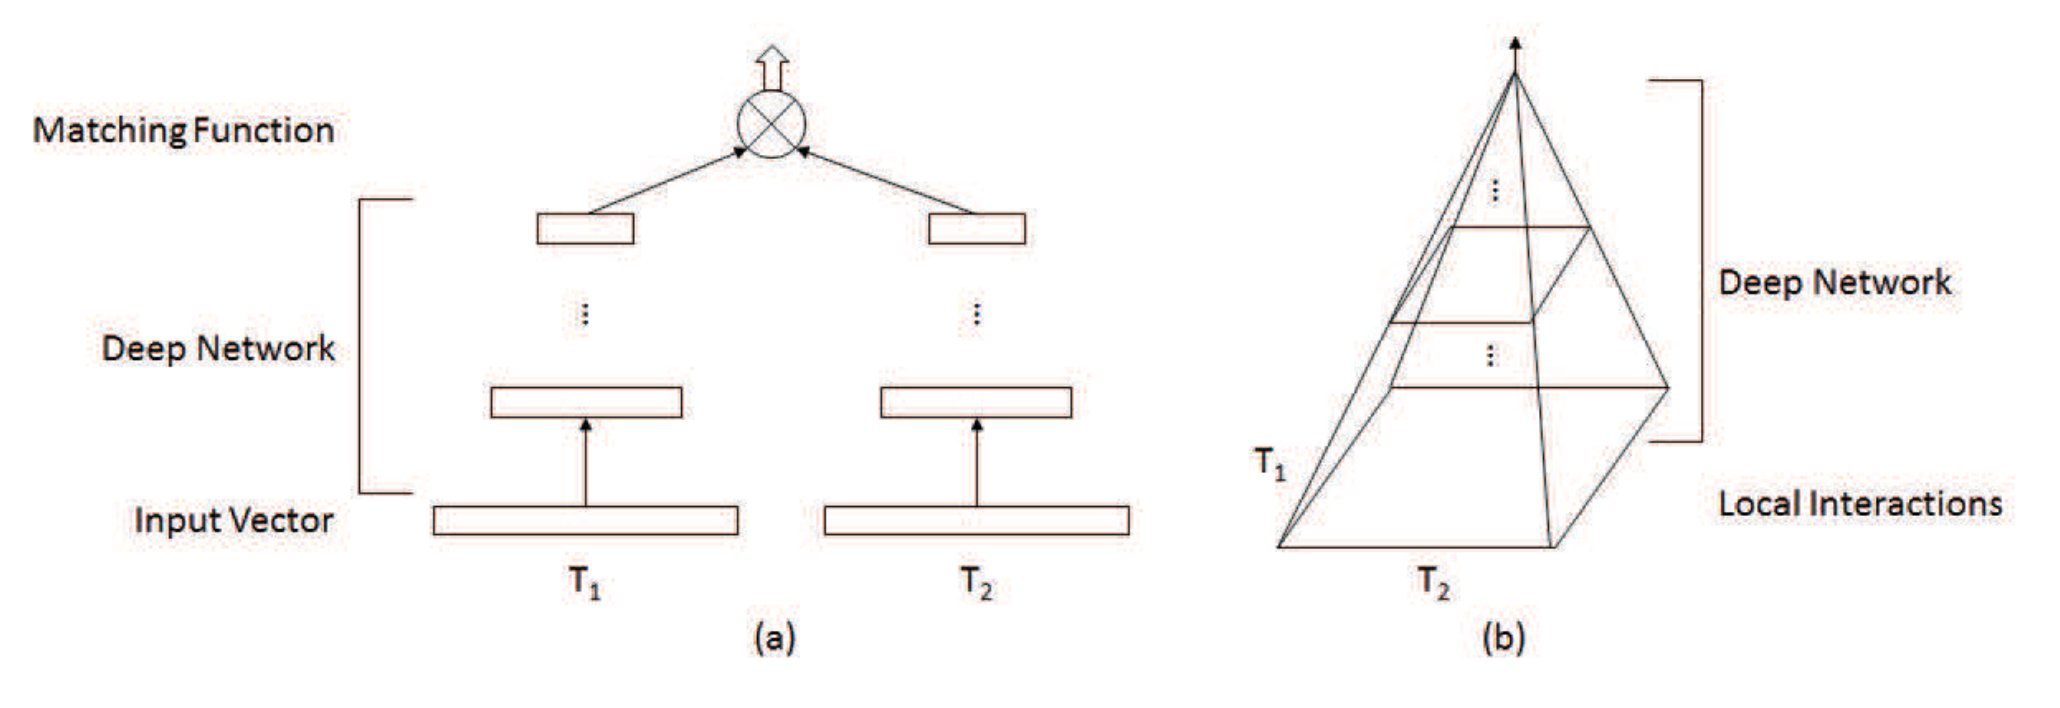
\includegraphics[width=6in]{deep_matching.png}
\caption{\cite{guo2017drmm}}
\label{fig:deep_matching}
\end{figure}

\myworries{concerns}
Neural models developed to address the deep matching problem can be divided into two broad categories based on their underlying architecture: representation-based and interaction-based.

\subsubsection{Representation-based Models}

Representation-based approaches first construct the representation from the input vectors for each text, e.g: documents, with a deep neural network, and then perform matching between the representations.
Earlier work on neural information retrieval focused on representation-based approaches, such as DSSM \cite{huang2013learning} and C-DSSM \cite{shen2014learning}.
DSSM (short for Deep Structured Semantic Models) \cite{huang2013learning} extended previously dominant latent semantic models to deep semantic matching for web search by projecting query and documents into a common low-dimensional space.
In order to accommodate a large vocabulary required by the task, the text sequences were mapped into character-level trigrams with a word hashing layer before computing a similarity matrix through dot product and softmax layers.
While shown effective on a private? datasset comprised of log files of a commercial search engine, DSSM was criticized by Guo et al. \cite{guo2017drmm} for requiring too much training data.
Moreover, DSSM cannot match synonyms because it is based on the specific composition of words.
C-DSSM \cite{shen2014learning} extended DSSM by introducing a convolutional layer to devise semantic vectors for search queries and Web document.
By performing a max pooling operation to extract local contextual information at the n-gram level, a global vector representation is formed from the local features.
They demonstrated that both local and global contextual features were necessary for semantic matching for Web search.
While C-DSSM improves over DSSM by exploiting the context of each trigram, it still suffers from the same issues listed above.
%However, ARC-I was mainly designed for short texts and ...

\subsubsection{Interaction-based Models}

Interaction-based approaches instead capture local matching signals, and directly compute the similarity of the query and document representations.
In contrast to more shallow representation-based approaches, in this approach deep neural network learns more complex hierarchical matching patterns.
Some notable examples include DRMM \cite{guo2017drmm}, KNRM \cite{xiong2017knrm} and DUET \cite{mitra2017neural}.
DRMM (stands for Deep Relevance Matching Model) \cite{guo2017drmm} maps the variable-length local interactions of each query term with the document? into a fixed-length matching histogram.
A feed forward matching network is used to learn hierarchical matching patterns and compute a matching score is computed for each term.
An overall matching score is obtained by aggregating the scores from each query term with a term gating network.
Similar to other models, KNRM \cite{xiong2017knrm} calculates the word-word similarities between query and document embeddings.
They propose a novel kernel-pooling technique to convert word-level interactions into ranking features.
\myworries{Details?}
Finally they combine the ranking features into a final ranking score through a learning-to-rank layer.
\myworries{Private dataset and stuff? Benefits?}
Unlike DRMM and KNRM, the goal of DUET \cite{mitra2017neural} is to employ both local and distributed representations to leverage both exact matching and semantic matching signals.
DUET is composed of two separate deep neural networks, one to match the query and the document using a one-hot representation, and another using learned distributed representations, which are trained jointly.
The former estimates document relevance based on exact matches of the query terms in the document by computing an interaction matrix from one-hot encodings.
The latter instead performs semantic matching by computing the element-wise product between the query and document embeddings.
Their approach was shown to significantly outperform traditional baselines for web search with lots of clickthrough logs.
%Mitra et al. \cite{mitra2017neural} show that distributed representations indeed improve over 
\myworries{Any other major models in the tutorial?}

%other models available in MatchZoo, such as ARC-I [9], MV-LSTM [19], and aNMM [21] were mainly designed for short texts and not geared towards handling documents (which are much longer)
%Note that some of the models discussed in this section address the web search task where a variety of other signals are available, such as large amounts of log data and the webgraph.
%This stands in contrast to the ``ad hoc'' document retrieval task where available data is limited only to the document text, which is the main focus of this thesis.
In fact, despite growing interest in neural models for document ranking, researchers have recently voiced concern as to whether or not they have truly contributed to progress~\cite{lin2019neural}, at least in the absence of large amounts of behavioral log data only available to search engine companies.
This opinion piece echoes the general skepticism concerning the empirical rigor and contributions of machine learning applications in Lipton et al. \cite{lipton2018troubling} and Sculley at al. \cite{sculley2018winner}.
%In particular, Lin et al.~\cite{lin2019neural} lament that comparisons to weak baselines sometimes inflate the merits of certain neural information retrieval methods.

To rigorously test this claim, Yang et al. \cite{Yang_etal_SIGIR2019} recently conducted a thorough meta-analysis of over 100 papers that report results on the TREC Robust 2004 Track.
Their findings are illustrated in Figure \ref{fig:neural_robust04} where the solid black line represents the best submitted run at 0.333, and the dotted black line the median TREC run at 0.258.
The other line is a RM3 baseline run with default parameters from the Anserini open-source information retrieval toolkit~\cite{Yang:2018:ARR:3289400.3239571} at AP 0.3903.
The untuned RM3 baseline is more effective than ~60\% of all studied papers, and ~20\% of them report results below the TREC median.
More surprisingly, only six of them report AP scores higher than the TREC best, with the highest being by Cormack et al.~\cite{Cormack:2009:RRF:1571941.1572114} in 2009 at AP 0.3686.
Among the neural models, the highest encountered score is by Zamani et al.~\cite{zamani2018neural} in 2018 at AP 0.2971.
%Despite the upward trend in the effectiveness of neural approaches, 

Yang et al. also implemented five recent neural retrieval models discussed above to evaluate their effectiveness on the ``ad hoc'' document retrieval task on the Robust04 dataset: DSSM, CDSSM, DRMM, KNRM and DUET.
These models were selected because they were specifically designed for ``ad hoc'' document retrieval unlike some others designed to handle shorter texts?
\myworries{All the models were trained on the documents in the baseline RM3 runs... details CV etc}
Table \ref{tab:exp-robust04} displays the AP and NDCG@20 values of each run on the Robust04 dataset.
The first two rows are taken from the original DRMM paper~\cite{guo2017drmm} and show their reported baseline and results; the other models do not report results on Robust04.
The next row refers to the untuned RM3 baseline from Anserini.
The following results refer to results from the neural models that were used to rerank the strong baseline, BM25+RM3, to gauge how much they actually contribute.
Of the five models, only one -- DRMM -- is found to significantly improve over the baseline.
%Mitra and Craswell [14] classified DRMM as a lexi- cal matching modeling (in fact, the model explicitly captures tfand idf). DUET is a hybrid lexical/semantic matching model, while the others are semantic matching primarily. One possible interpretation of our findings is that TREC judgments alone are not sufficient to train semantic matching models

\begin{table}[t]
\vspace{0.2cm}
\centering
\begin{tabular}{lll}
\toprule
\textbf{Condition} \mbox{\hspace{0.5cm}} & \textbf{AP} \mbox{\hspace{1.0cm}} & \textbf{NDCG@20} \\ 
\toprule
BM25~\cite{guo2016deep} & 0.255 & 0.418 \\
DRMM~\cite{guo2016deep} & 0.279 & 0.431 \\
%Paper 2    & 0.272       & - \\
BM25+RM3   & 0.3033      & 0.4514     \\
~+ DSSM    & 0.3026      & 0.4491     \\  
~+ CDSSM   & 0.2995      & 0.4468     \\
~+ DRMM    & 0.3152$^{\dagger}$  & 0.4718$^{\dagger}$ \\  
~+ KNRM    & 0.3036      & 0.4441     \\  
~+ DUET    & 0.3051      & 0.4502     \\ 
\bottomrule
\end{tabular}
\vspace{0.2cm}
\caption{Experimental results applying neural models to rerank a strong baseline; $^{\dagger}$ indicates statistical significance.}% at the $p<0.01$ level.}
\label{tab:exp-robust04}
\vspace{-0.6cm}
\end{table}

\begin{figure}[b!]
\centering
  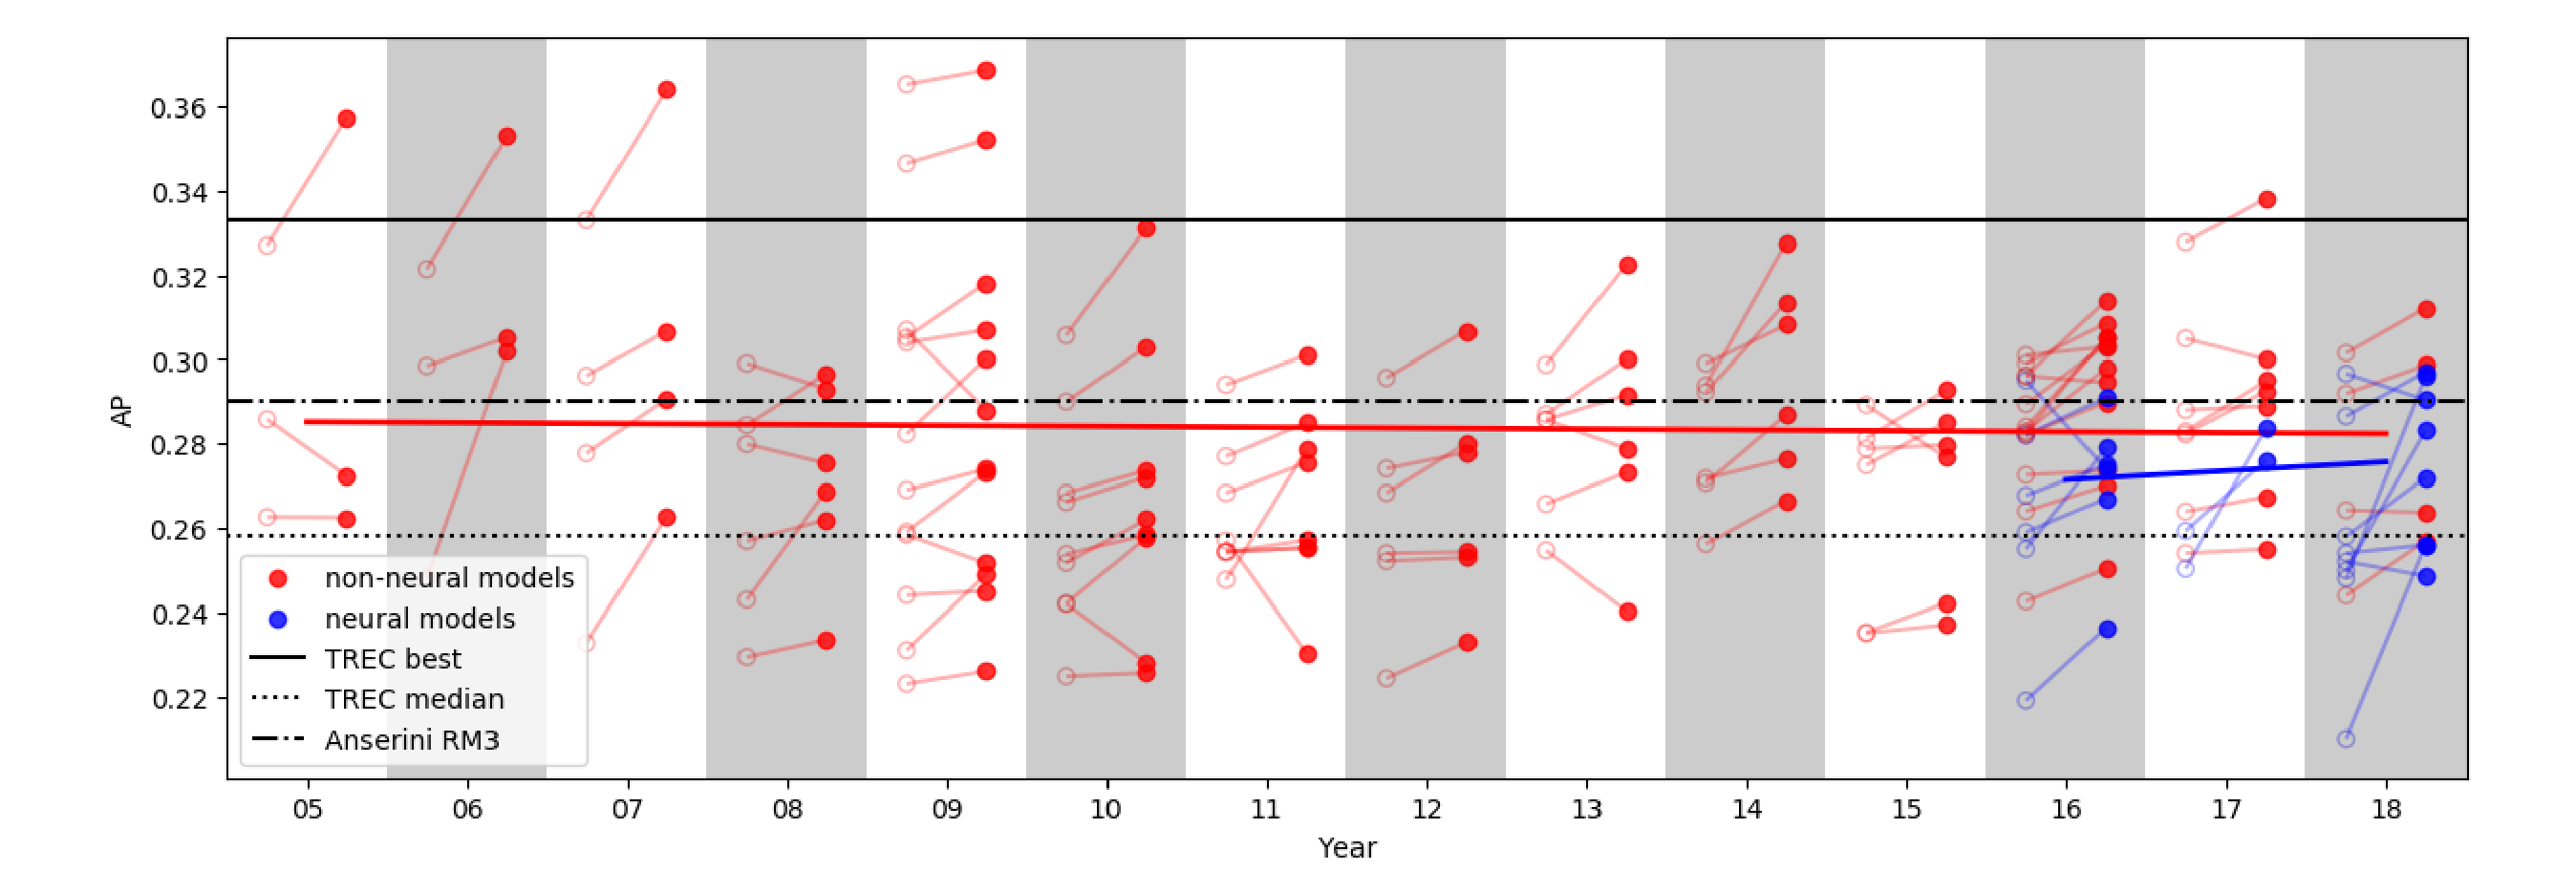
\includegraphics[width=6in]{neural_robust04.png}
\caption{...}
\label{fig:neural_robust04}
\end{figure}

\subsubsection{Contextualized Language Models}

While the neural ranking models introduced in the previous section successfully leverage contextual information to improve retrieval effectiveness, they are limited by the size and variability of the available training data.
Ideally, these models would be trained on a large number of semantically varied yet relevant query-document pairs; however, it is impractical to automatically gather a sufficient number of such training samples.
Massively pretrained unsupervised language models hold promises for obtaining better representations for the query and document, and therefore, achieving unprecedented effectiveness at semantic matching without the need for more relevance information.
Language models are pretrained on massive amounts of external data in an unsupervised fashion.
\myworries{ELMo, GPT, BERT...}

Document retrieval requires an understanding of the relationship between two text sequences -- the query and the document.
However, language modeling does not suffice to capture such a relationship.
BERT facilitates such relevance classification by pre-training a binary next sentence prediction task based on its masking language model approach.
This mechanism has been adopted for ``passage'' reranking by ...
Notably, Nogueira et al. \cite{nogueira2019passage} proposed to re-rank MS MARCO passages based on a simple re-implementation of BERT, outperforming the previous state of the art by 27\% in MRR@10 and replacing the top entry in the leaderboard of the MS MARCO passage retrieval task at the time of publication.
Our neural model is inspired by the BERT re-implementation described in this paper.
\myworries{What about others? MS MARCO leaderboard?}

To our knowledge, Yang et al. \cite{yang2019simple} were the first to successfully apply BERT to ``ad hoc'' document retrieval.
They demonstrated that BERT can be fine-tuned to capture relevance matching by applying the above approach on the TREC Microblog Tracks where document length does not pose an issue.
They further proposed overcoming the challenge of long documents by applying inference on each individual sentence and combining the top scores to compute a final document score.
Their approach was motivated by user studies? by Zhang et al. \cite{zhang2018effective} who suggested that the most relevant sentence or paragraph in a document provides a good proxy for overall document relevance.
Their work paved the way for future work that culminated in this thesis.

More recently, MacAvaney et al. \cite{macavaney2019cedr} shifted focus from incorporating BERT as a reranker to using its representation capabilities to improve existing neural architectures.
By computing a relevance matrix between the query and each candidate document? at each layer of a contextualized language model -- ELMo or BERT --  they established state-of-the-art effectiveness on Robust04 and Webtrack 2012--2014 at the time of writing.
\myworries{Not MAP...}
They also proposed a joint model that combines the aforementioned classification mechanism of BERT into existing neural architectures.
They claim that this approach benefits from both deep semantic matching with BERT \textit{and} relevance batching with traditional ranking architectures.

Qiao et al. \cite{Qiao:1904.07531:2019} study in an arXiv preprint the performance and behavior of BERT when used as a reranker for passage ranking on MS MARCO and for document ranking on the TREC Web Track.
Their findings are consistent with those of Nogueira et al. \cite{nogueira2019passage} in that BERT outperforms previous neural models on the passage reranking task on MS MARCO.
For ad hoc document ranking, they explore using BERT as representation-based and interaction-based rankers and in combination with some of the neural models discussed in Section \myworries{X}.
\myworries{However, they find that BERT, even when pretrained on MS MARCO ranking labels, performs worse than feature-based learning to rank and neural retrieval models pretrained user clicks in Bing log.}	
They also compare their BERT-based reranker to Conv-KNRM \cite{dai2018convolutional}.
Compared to interaction-based neural models that focus on term pairs, they show that BERT propagates information across larger spans through its attention mechanism.

Padigela et al. \cite{Padigela:1905.01758:2019} also focus on understanding the reasons behind the gains on passage reranking on MS MARCO.
They also demonstrate that fine-tuning BERT is more effective than feature based learning to rank models such as RankSVM \cite{joachims2002optimizing} and a number of neural kernel matching models such as KNRM \cite{xiong2017knrm} and Conv-KNRM \cite{dai2018convolutional}.
They test four hypotheses regarding the behavior of semantic matching with BERT compared to BM25; specifically, with respect to term frequency and document length.
\myworries{More?}

\section{Evaluation Metrics}

The standard approach to evaluation in information retrieval relies on the distinction between ``relevant'' and ``irrelevant'' documents with respect to an information need as expressed by a query.
A number of automatic evaluation metrics has been formalized for ranking tasks such as document retrieval.
These metrics rely on 
The size of most document collections makes it infeasible for humans to manually judge the relevance of all documents.
All relevant documents need to be labelled to prevent false negatives, i.e: treating documents which are in fact relevant as irrelevant.

\subsection{Mean Average Precision (MAP)}

Precision specifies what fraction of a set of retrieved documents is in fact relevant for a given query $ q $.
Precision can easily be extended to evaluate ranked retrieval results by ...
Average precision (AP) expresses the average of the precision values obtained for the set of top $ k $ documents for a query.
Support that $ D = \{d_1, ..., d_{m_j}\} $ is the set of all relevant documents for a query $ q_j $, then AP can be formulated as:

\begin{equation}
AP = \frac{1}{m_j} \sum^{m_j} _{k = 1} P(R_{jk})
\end{equation}

where $ R_{jk} $ represents the set of top $ k $ tanked retrieval results.

The respective AP for each query can be aggregated to obtain mean average precision (MAP) for the overall retrieval effectiveness in the form of a single-figure measure of quality across various recall levels:

\begin{equation}
MAP = \frac{\sum^{|Q|} _{j = 1} AP}{Q} = \frac{1}{Q} \sum^{|Q|} _{j = 1} \frac{1}{m_j} \sum^{m_j} _{k = 1} P(R_{jk})
\end{equation}

%\myworries{Meaning of MAP: To recapitulate, if the AP is 0.5, the relevant
%answer occurs at every second position. If the AP score is 0.3, the relevant answer occurs
%at every 3rd position and an AP score of 0.1 would mean that every 10th answer is correct.}

It has been show to have especially good discrimination and stability compared to other metrics, which makes it the ideal choice for large text collections \cite{manning2010introduction}.
It is hence one of the standard metrics among the TREC community.

\subsection{Precision at k (P@k)}

Unlike MAP which factors in precision at all recall levels, certain applications have a distinctly different notion for ranking quality.
Particularly in the case of web search, the user often only cares about the results on the first page or two, but not all of them.
This restriction essentially leads to measuring precision at fixed low levels of retrieved results, i.e: top $ k $ documents -- hence the name for metric ``precision at $ k $''.
On the one hand, it eliminates the need for any estimate of the size of the set of relevant documents.
However, it also produces the least stable out of all measures.
Moreover, precision at $ k $ does not average well because the total number of relevant documents for a query has a very strong influence on its value. 

\subsection{Normalized Discounted Cumulative Gain (NDCG@20)}

Cumulative gain (CG) simply computes the sum of relevance labels for all the retrieved documents.
It views the search results as an unordered set, and disregards the ordering of the documents.
Since a highly relevant document is inherently more useful when it appears higher up in the search results, CG has been extended to discounted cumulative gain (DCG).
Discounted cumulative gain (DCG) estimates the relevance of a document based on its rank among the retrieved documents.
The relevance measure is accumulated from top to bottom, discounting the value of documents at lower ranks.
NDCG measures DCG for the top $ k $ documents, normalizing by the highest possible value for a query.

NDCG is uniquely useful in applications with a non-binary notion of relevance, e.g: a spectrum of relevance. 
For this reason, NDCG is a popular choice for systems with machine learning approaches?
Like precision at k, it is evaluated as a weighted sum over the top k search results, and normalized so that a perfect ranking yields NDCG equals 1.
This makes NDCG comparable across different queries:\
The NDCG values for all queries can be averaged to reliably evaluate the effectiveness of a ranking algorithm for various information needs across a collection.
However, the use of NDCG is dependent on the availability of ground truth relevance labels?